% Kompiuterijos katedros šablonas
% Template of Department of Computer Science II
% Versija 1.0 2015 m. kovas [ March, 2015]

\documentclass[a4paper,12pt,fleqn]{article}
\usepackage[unicode,colorlinks=false]{hyperref}


\usepackage[utf8x]{inputenc}
%

\usepackage[L7x]{fontenc}
\usepackage{times}
\usepackage{ucs}

 %package to switch the language
\usepackage{etoolbox}

  %set up of the page margins
\usepackage[top=2cm, bottom=2cm, left=3cm, right=1.5cm]{geometry}

 %1.1 line spacing
\linespread{1.1}


  %page numbering at the right side
\usepackage{fancyhdr}
\pagestyle{fancyplain}
\fancyhf{}
\renewcommand{\headrulewidth}{0pt} 
\fancyhfoffset[RO]{0cm}

  %to number at the bottom (exchange lines to number at the top)
\rfoot{\thepage}
  %\rhead{\thepage} %

% \usepackage[usenames,dvipsnames]{pstricks}
\urlstyle{same}
\hypersetup{
%  citecolor=Blue,
%  linkcolor=Blue,
%  urlcolor=Blue
pdfborder={0 0 0 }
}

 %for includegraphics
\usepackage{graphicx}



\usepackage[toc,page]{appendix}


\usepackage{caption}

 %for source codes
\usepackage{listings}
\lstset{commentstyle=\color{red},xleftmargin=10pt, framexleftmargin=6pt, numbersep=1mm, frame=single, numbers=left,numberstyle=\footnotesize,extendedchars=\true, inputencoding=utf8x,basicstyle=\footnotesize,extendedchars=true,
 keywordstyle=\color{black}\bfseries, breaklines=true, breakautoindent=true,framesep=8pt,linewidth=0.95\textwidth
}

 %for algorithms
\usepackage{algorithm}
\usepackage{algorithmic}
 %instead of the above two packages we can use algorithms2e
 %\usepackage[boxed,linesnumbered,vlined,slide]{algorithm2e}

 %special symbols
\usepackage{amsfonts}
\usepackage{amssymb}
\usepackage{amsmath}

 %for theorem like environments
\usepackage{amsthm}

 \usepackage{datetime}
 \renewcommand{\dateseparator}{--}


% SI system units
\usepackage{siunitx}
\sisetup{detect-all}
% Problem with fonts \SI{x.xx}{\micro\metre}, solved with updmap-sys --enable Map=utm.map
\renewcommand{\sfdefault}{uhv}
\renewcommand{\rmdefault}{utm}
\renewcommand{\ttdefault}{ucr}

% List management (itemize, etc.)
\usepackage{enumitem}

\newcommand*{\urlw}[1]{\href{#1}%
            {\nolinkurl{#1}}}


\newtoggle{inLithuanian}
%If the report is in Lithuanian, it is set to true; otherwise, change to false
\settoggle{inLithuanian}{true}

%create file preface.tex for the preface text
%if preface is needed set to true
\newtoggle{needPreface}
\settoggle{needPreface}{false}

\newtoggle{signaturesOnTitlePage}
\settoggle{signaturesOnTitlePage}{false}



\theoremstyle{definition}
\newtheorem{definition}{\keyWordDefinition}
\newtheorem{example}{\keyWordExample}
\def\QED{\unskip\nobreak\hfill\kern5pt$\Box$}

\iftoggle{inLithuanian}{
%\usepackage[L7x]{fontenc}
\usepackage[english,lithuanian]{babel}

\newcommand{\todayiso}{\the\year \dateseparator \twodigit\month \dateseparator \twodigit\day}


\renewcommand{\today}{\number\year\space m. \space \ifcase\month\or
  sausio\or vasario\or kovo\or balandžio\or gegužės\or birželio\or
  liepos\or rugpjūčio\or rugsėjo\or spalio\or lapkričio\or
  gruodžio\fi
  \space\number\day\space d.}


 \usepackage{tocloft}
 \renewcommand\cftsecaftersnum{.} 
 \renewcommand\cftsubsecaftersnum{.} 
 \renewcommand\cftsubsubsecaftersnum{.}

 \usepackage{VUMIFKK}

 \DeclareCaptionLabelFormat{captionlt}{#2 #1}
   %smth is not fine with algorithms 
 \DeclareCaptionLabelFormat{captionltalg}{#2 #1 algoritmas}

 \usepackage{indentfirst}
 \renewcommand{\appendixtocname}{Priedai}
 \renewcommand{\appendixpagename}{Priedai}
 \renewcommand{\contentsname}{Turinys} 

 \renewcommand{\lstlistingname}{išeities kodas}
 \renewcommand{\figurename}{pav}
 \renewcommand{\tablename}{lentelė}


 \captionsetup*[lstlisting]{   
 labelsep=period,labelformat=captionlt
 }
 \captionsetup*[figure]{   
% labelsep=period,
 labelsep=space, %babel redefines pav to pav.
 labelformat=captionlt
 }
 \captionsetup*[table]{   
  labelsep=period,
  labelformat=captionlt
 }
 \renewcommand{\algorithmicrequire}{\textbf{Įvestis:}}
 \renewcommand{\algorithmicensure}{\textbf{Išvestis:}}

 \captionsetup*[algorithm]{   
 labelsep=period,labelformat=captionltalg
 }

\renewcommand{\thmhead}[3]{#2 #1#3}

}
{
%\usepackage[OT1,T1]{fontenc}
%\usepackage[L7x]{fontenc}

\usepackage[english]{babel}
\newcommand{\todayiso}{\twodigit\month \dateseparator \twodigit\day \dateseparator \the\year}
 \captionsetup*[algorithm]{   
 labelsep=period
 }
\captionsetup*[lstlisting]{   
 labelsep=period
 }
 \captionsetup*[figure]{   
 labelsep=period
 }
 \captionsetup*[table]{   
 labelsep=period
 }


}

%some kywords
 \def\keywordAbstract{\iftoggle{inLithuanian}{Santrauka}{Abstract}}
 \def\keywordAbstractOther{\iftoggle{inLithuanian}{Summary}{Santrauka}}
 \def\keyWordIntroduction{\iftoggle{inLithuanian}{Įvadas}{Introduction}}
 \def\keyWordConclusions{\iftoggle{inLithuanian}{Išvados}{Conclusions}}

 \def\keyWordPreface{\iftoggle{inLithuanian}{Pratarmė}{Preface}}
 \def\keyWordAppendice{\iftoggle{inLithuanian}{Priedas}{Appendix}}
 \def\keyWordSignature{\iftoggle{inLithuanian}{parašas}{signature}}
 \def\keyWordDefinition{\iftoggle{inLithuanian}{apibrėžimas}{Definition}}
 \def\keyWordExample{\iftoggle{inLithuanian}{pavyzdys}{Example}}

\newcommand{\bothabstracts}[3]{
\setcounter{secnumdepth}{0}
\newpage
\hspace{2cm}
{\centering{\section{\keywordAbstract}}}

#1
\newpage
\hspace{2cm}
{\centering \section{\keywordAbstractOther}}

\begin{center}{\textbf{#2} }\end{center}

 #3
\setcounter{secnumdepth}{3}
}

 %non-numbered sections: #1 param: for labeling sec:#1, #2 -section title
\newcommand{\sectionWithoutNumber}[2]{\newpage
%\hspace{2cm}
\section*{#1}
\label{sec:#2}
\addcontentsline{toc}{section}{\nameref{sec:#2}}%{#3}
 }



\newcommand{\referenceSources}[1]{
\newpage
\cleardoublepage
\phantomsection
\iftoggle{inLithuanian}{
 \renewcommand{\refname}{Literatūros šaltiniai}

 \addcontentsline{toc}{section}{Literatūros šaltiniai}
 \markboth{\refname}{Literatūros šaltiniai}
 }
{

\addcontentsline{toc}{section}{References}
\markboth{References}{References}
}

\bibliographystyle{plain}
\bibliography{#1}
}



 \newcommand\authorsignature[1]{
\begin{flushright}
 \begin{minipage}[b]{0.45\textwidth}
  \centering
  \rule{\textwidth}{0.5pt}\\
   #1
  \end{minipage}
\end{flushright}
 }




 \newcommand\authorsignatures[5]{%
   \vspace{1cm}
   \authorsignature{#1}
   \ifstrequal{#2}{}{}{\vspace{0.3cm}
     \authorsignature{#2}
     \ifstrequal{#3}{}{}{\vspace{0.3cm}
      \authorsignature{#3}
      \ifstrequal{#4}{}{}{\vspace{0.3cm}
        \authorsignature{#4}
        \ifstrequal{#5}{}{}{\vspace{0.3cm}
         \authorsignature{#5}       
        }
      }
    }
} 
}

\newcommand{\authortitle}{
\iftoggle{signaturesOnTitlePage}{
\tiny{\keyWordSignature}
}{}
}

\newcommand{\depttitlepage}[8]
{
\thispagestyle{empty}
\begin{center}


\includegraphics[width=2cm]{jb_VU_zenklas}

%\vspace{-1cm}

\iftoggle{inLithuanian}
{ 
  VILNIAUS UNIVERSITETAS\\
  MATEMATIKOS IR INFORMATIKOS FAKULTETAS\\
  KOMPIUTERIJOS KATEDRA
}
{
  VILNIUS UNIVERSITY \\
  FACULTY OF MATHEMATICS AND INFORMATICS \\
  DEPARTMENT OF COMPUTER SCIENCE II
}

\vspace{5cm}

#1\\
\vspace{0.5cm}
\textbf{\Large #2}
\end{center}

\vspace{5cm}


\hspace{0.5\textwidth}
\begin{minipage}{0.4\textwidth}
 \begin{flushleft} 
\iftoggle{inLithuanian}
{
 \ifstrequal{#3}{}{}{Atliko:\\[5pt]}
}
{
\ifstrequal{#3}{}{}{Done by:\\[5pt]}
}

%\noindent
\begin{tabular}{@{}lr}%\setlength\tabcolsep{0pt}
\ifstrequal{#3}{}{}{#3&\hspace{2cm}\authortitle\\[5pt]}
\ifstrequal{#4}{}{}{#4&\authortitle\\[5pt]}
\ifstrequal{#5}{}{}{#5&\authortitle\\[5pt]}
\ifstrequal{#6}{}{}{#6&\authortitle\\[5pt]}
\ifstrequal{#7}{}{}{#7&\authortitle\\}
\end{tabular}

\end{flushleft}

\end{minipage}

\vspace{0.5cm}
\hspace{0.5\textwidth}
\begin{minipage}{0.4\textwidth}
 \begin{flushleft} 

\ifstrequal{#8}{}{}
{

\iftoggle{inLithuanian}
{
Vadovas:
}
{
Supervisor:
}

#8

}

\end{flushleft}

\end{minipage}


\vfill

\begin{center}
Vilnius\\
\the\year
\end{center}

\iftoggle{needPreface}{
 \sectionWithoutNumber{\keyWordPreface}{preface}
\input{preface.tex}

\iftoggle{inLithuanian}
{
\vspace{\baselineskip}\hfill
\today
}
{
 \vspace{\baselineskip}\hfill \today
}

 \vspace{5cm}

\iftoggle{signaturesOnTitlePage}{}
{
\authorsignatures{#3}{#4}{#5}{#6}{#7}
}
}{}
\newpage
}


\begin{document}
    % #1 -report type, #2 - title, #3-7 students, #8 - supervisor
    \depttitlepage{Pirma užduotis}{Signalų poros tarpusavio koreliacija}{Edvinas Naraveckas}
    {}{}{}{}% students 2-5
    {}

    \tableofcontents

    %Introduction section: label is sec:intro
    \sectionWithoutNumber{\keyWordIntroduction}{intro}
    Darbe nagrinėjamos šešios signalų poros ir jų tarpusavio koreliacija.
Užduotis atlikta \textit{Haskell} kalba. Grafikai gauti naudojant \textit{Gnuplot} įrankį.

Jei turme diskrečius signalus \(f(t)\) ir \(g(t)\) kurių laiko trukmė \(t\) yra lygi
ir abiejų signalų diskretizavimo žingsnis \(\Delta t\) yra tas pats,
tai signalų tarpusavio koreliacija apibrėžiama funkcija:

\begin{equation}
    r_{fg} (d) = \dfrac{\displaystyle \sum\limits_{j=0}^{N-d} {(f_j - \bar{f}) (g_{d+j} - \bar{g})}} {\sqrt{\displaystyle \sum\limits_{j=0}^{N-d} (f_j - \bar{f})^2 \displaystyle \sum\limits_{j=0}^{N-d} (g_{d+j} - \bar{g})^2}},\qquad
    d = 0,1, \ldots\ ,[N/2].
\end{equation}

čia

\begin{equation}
    \bar{f} = \dfrac{1} {N-d+1} \displaystyle \sum\limits_{i=0}^{N-d} {f_i},\qquad
    \bar{g} = \dfrac{1} {N-d+1} \displaystyle \sum\limits_{i=0}^{N-d} {g_{d+i}}.
\end{equation}

Parametras \(d\) yra poslinkis laike.
Tai yra, per kiek diskretaus laiko žingsnių yra pastumtos \(g\) reikšmės \(f\) reikšmių atžvilgiu.

Jei sukeičiame \(f\) ir \(g\) reikšmes, galime skaičiuoti neigiamą signalų koreliacią, arba į praeitį.
kas iš tiesų parodo ar \(g\) kitimas turėjo įtakos \(f\) reikšmėms.
Funkciją \(r_{gf}\) galima interpretuoti kaip \(r_{fg}\) funkcijos pratesimą į neigiamas \(d\) reikšmes:

\begin{equation}
    r_{fg} (d) = r_{gf} (|d|),\qquad d = 0,-1, \ldots\ ,-[N/2].
\end{equation}

Grafikas pagal \(d\) nėra pakankamai informatyvus, nes reikia žinoti diskretaus laiko žingsį.
Geresnis būdas atvaizduoti signalų tarpusavio koreliaciją yra naudojant priklausomybę nuo realaus laiko \(t\).
Tuomet signalų koreliacijos funkcija nuo \(t\) žymėsime \(R_{fg}(t)\):

\begin{equation}
    R_{fg} (t) = r_{fg} (d),\qquad t = d\Delta t,\qquad d = -[N/2],-[N/2]+1, \ldots\ ,0,1, \ldots\ ,[N/2].
\end{equation}

Signalų tarpusavio koreliacijos grafikas \(R_{fg}(t)\) rodo signalų panašumą.
Jo rezultatus galima interpretuoti suskirsčius gautas reikšmes intervalais:

\begin{itemize}
    \item Visiems \(t, |R_{fg}(t) \in [0, 0.2]\): tarp signalų \textit{nėra} statistinio panašumo arba jis labai silpnas.
    \item Tam tikriems \(t, |R_{fg}(t) \in (0.2, 0.5]\): tarp signalų yra \textit{silpnas} statistinis ryšys.
    \item Tam tikriems \(t, |R_{fg}(t) \in (0.5, 0.7]\): tarp signalų yra \textit{vidutinis} statistinis ryšys.
    \item Tam tikriems \(t, |R_{fg}(t) \in (0.5, 1]\): tarp signalų yra \textit{stiprus} statistinis ryšys.
\end{itemize}

O, maksimali \(t\) reikšmė parodo per kiek reikėtų pastumti \(g\) reikšmes, kad jie taptų labiausiai panašūs.


    %the main part
    \section{Karo pabėgėliai ir „war“ žodžio dažnumas antraštėse}
    \label{sec:refugees}
    Karo pabėgėliu mėnesinis skaičius pagal šalis\cite{refugees} buvo sutrauktas į bendrą per mėnesinį pasaulio babėgėlių skaičių 2003 - 2017 metais.
Žodžio „war“ skaičius per mėnesį buvo surinktas iš ABC naujienų portalo antraščių\cite{abcNews} tuo pačiu laikotarpiu.

\begin{figure}
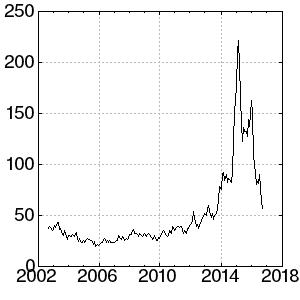
\includegraphics[scale=0.65]{../scripts/refugees_war/refugees.png}
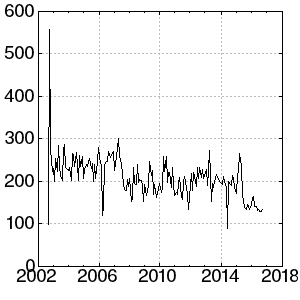
\includegraphics[scale=0.65]{../scripts/refugees_war/war.png}
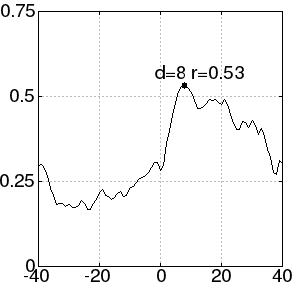
\includegraphics[scale=0.65]{../scripts/refugees_war/result.png}
    \caption{Grafikas kairėje: vidutinis mėnesinis karo pabėgėlių skaičius pasaulyje (tūkstančiais). Grafikas centre: mėnesinis „war“ skaičius ABC naujienų antraštėse. Grafikas dešinėje: signalų tarpusavio koreliacija}
\end{figure}

Nors tarp karo pabėgėlių ar žodžio „war“ dažnumo grafiko akivaizdaus ryšio nesimato,
poros koreliacijos funkcija rodo didžiausią signalų panašumą \( R_{fg}(t) = 0.53 \), kai \( t = 8 \).
Signalų porą galima klasifikuoti kaip vidutiniškai koreliuojančia tarpusavyje.
Koreliacijos grafikas parodo, kad didžiausias pabėgėlių skaičius fiksuojamas praėjus vidutiniškai aštuoniems mėnesiams po didžiausio žiniasklaidos susidomėjimo.
Žodžio „war“ dumenys gali būti klaidinantys ir iškreipiantys tikrąją koreliaciją, nes neįvertina klaidingų sutapimų (false positives), kaip dažnai naudojamas angliškas posakis „war on drugs“ ir pan.
Taip pat,rezultatus būtų galima patikslinti, atrinkus antraštes su „war“ ir šalies pavadinimu, ir patikrinus koreliaciją su pabėgėlių skaičiumi iš tos šalies.


    \section{Užtriukšminti karo pabėgėlių ir „war“ žodžio dažnumo signalai}
    \label{sec:noisy-refugees}
    Užtriukšminti karo pabėgėlių ir žodžio „war“ skaičius per mėnesį signalai (~\ref{fig:noisy} pav.) gauti panaudojus paprastą atsitiktinių skaičių (random) generatorių \(y = x * rand\), kai \(rand\) generuoja reikšmes iš \((0, 1)\). Tada, pakeičiant švarų signalą užtriukšmintu, paskaičiuota signalų tarpusavio koreliacija.

\begin{figure}
    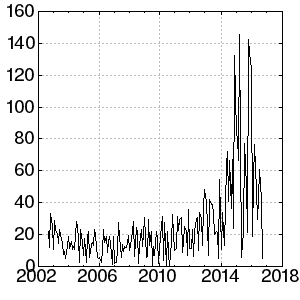
\includegraphics[scale=0.65]{../scripts/refugees_war_rand/refugees_rand.png}
    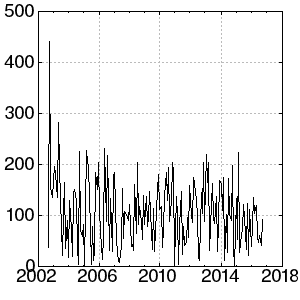
\includegraphics[scale=0.65]{../scripts/refugees_war_rand/war_rand.png}
    \caption{Grafikas kairėje: užtriukšmintas bendras mėnesinis karo pabėgėlių skaičius pasaulyje (tūkstančiais). Grafikas dešinėje: užtriukšmintas mėnesinis „war“ žodžio dažnumas ABC naujienų antraštėse.}
    \label{fig:noisy}
\end{figure}

\begin{figure}
    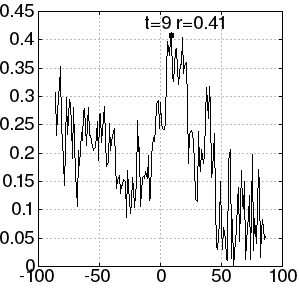
\includegraphics[scale=0.65]{../scripts/refugees_war_rand/result_ref_rand.png}
    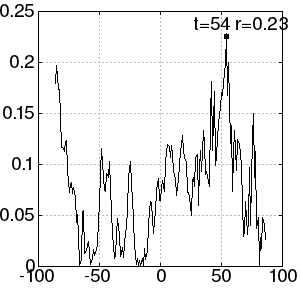
\includegraphics[scale=0.65]{../scripts/refugees_war_rand/result_war_rand.png}
    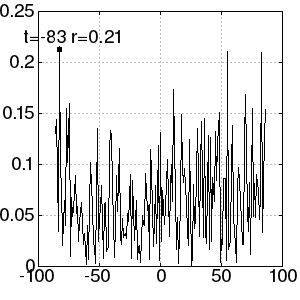
\includegraphics[scale=0.65]{../scripts/refugees_war_rand/result_both_rand.png}
    \caption{Grafikas kairėje: užtriukšminto pabėgėlių ir švaraus „war“ dažnumo koreliacija. Grafikas centre: švaraus pabėgėlių ir užtriukšminto „war“ dažnumo koreliacija. Grafikas dešinėje: signalų tarpusavio koreliacija kai abu signalai užtiukšminti.}
    \label{fig:noisy_cross}
\end{figure}

Iš koreliacijos grafikų (~\ref{fig:noisy_cross} pav.) matosi, kad užtriukšmintas pabėgelių skaičius nestipriai pakeitė algoritmo rezultatus.
Bet tokiu pačiu metodu užtriukšmintas „war“ žožio dažnumas daug stipririau iškreipė koreliacijos grafiką, kai pabėgėlių signalas buvo švarus.
Užtriukšminus abu signalus, algoritmas neberanda vidutinės koreliacijos tarp jų ir grafike matosi atsiradę keletas naujų lokalių maksimumų.


    \section{Saulės dėmių skaičius ir vidutinės temperatūros anomalijos}
    \label{sec:sunspots}
    Vidutinis mėnesinis saulės dėmių skaičius\cite{sunspots} 1880 - 2016 metais.
Globalios mėnesinės temperatūros vidutinės anomalijos\cite{temp} tuo pačiu laikotarpiu.

\begin{figure}
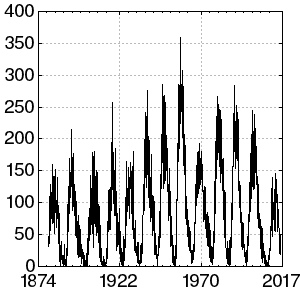
\includegraphics[scale=0.65]{../scripts/sunspots_temperature/sunspots.png}
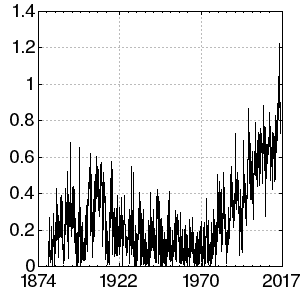
\includegraphics[scale=0.65]{../scripts/sunspots_temperature/temp.png}
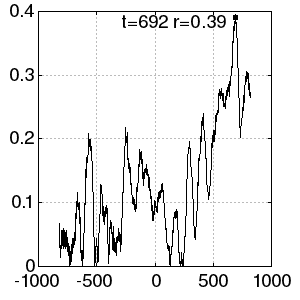
\includegraphics[scale=0.65]{../scripts/sunspots_temperature/result.png}
\caption{Grafikas kairėje: vidutinis mėnesinis saulės dėmių skaičius. Grafikas centre: globalios mėnesinės temperatūros vidutinės anomalijos. Grafikas dešinėje: signalų tarpusavio koreliacija.}
\end{figure}

Signalų poros koreliacijos funkcija rodo didžiausią signalų panašumą \( R_{fg}(t) = 0.39 \), kai \( t = 692 \).
\( R_{fg}(t)\) rodo labai silpną statistinį ryšį. O, \(t\) yra 692 mėnesiai, tai yra apie 57 metų poslinkis.
Esant tokiems rezultatams galima konstatuoti, kad koreliacijos tarp saulės aktyvumo ir temperatūros anomalijų nėra arba reikia smulkesnės analizės.
Panašias išvadas pateikia kitas tyrimas\cite{temp_study}.
Saulės aktyvumas kinta periodiškai kas vienuoliką metų. Poslinkis \(t\) turėtų būti \(< 122 \) mėnesių.


    \section{Aukso ir naftos kainos}
    \label{sec:oil-gold}
    \begin{figure}
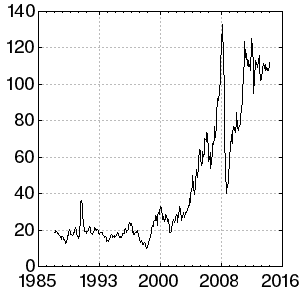
\includegraphics[scale=0.65]{../scripts/oil_gold/oil.png}
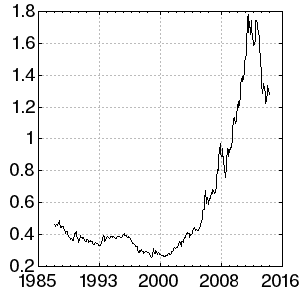
\includegraphics[scale=0.65]{../scripts/oil_gold/gold.png}
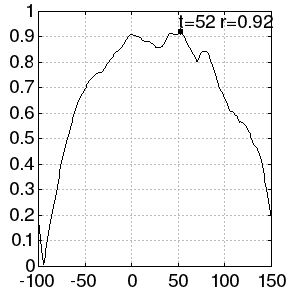
\includegraphics[scale=0.65]{../scripts/oil_gold/result.png}
    \caption{Grafikas kairėje: vidutinė mėnesinė naftos kaina už barelį (USD). Grafikas centre: vidutinė mėnesinė aukso kaina (tūkstančiais USD). Grafikas dešinėje: signalų tarpusavio koreliacija}
\end{figure}

Tirama brent naftos vidutinė mėnesinė kainos\cite{oil} 1987 - 2014 metais koreliacija su aukso mėnesinė vidutine kaina\cite{gold} tuo pačiu laikotarpiu.
Signalų tarpusavio koreliacijos grafikas rodo stiprių ryšį ir turi kelias pagal reikšmę artimas viršūnes.
Didžiausias signalų panašumas yra kai \( R_{fg}(t) = 0.92 \) ir \( t = 52 \).
Bet kitas didelis statistinis panašumas yra kai \( R_{fg}(t) = 0.91 \) ir \( t = 0 \).



    \section{JAV gimstamumas ir BVP}
    \label{sec:gdp-births}
    Jungtinių Amerikos Valstijų bendras vidaus produktas\cite{gdp} 1987 - 2014 metais ir
Jungtinių Amerikos Valstijų gimstamumas\cite{births} tuo pačiu laikotarpiu.
Gimstamumo per mėnesį duomenys buvo akumuliuoti į metinius.

\begin{figure}
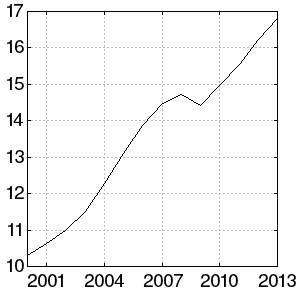
\includegraphics[scale=0.65]{../scripts/gdp_births/gdp.png}
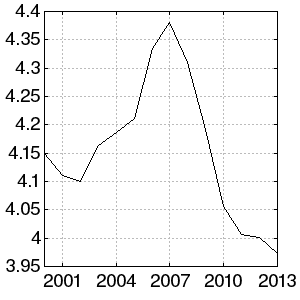
\includegraphics[scale=0.65]{../scripts/gdp_births/births.png}
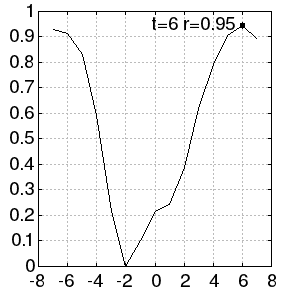
\includegraphics[scale=0.65]{../scripts/gdp_births/result.png}
    \caption{Grafikas kairėje: JAV BVP (trln. USD). Grafikas centre: naujagimių skaičius per metus (milijonais). Grafikas dešinėje: signalų tarpusavio koreliacija}
\end{figure}

Signalų tarpusavio koreliacijos grafikas rodo stiprių ryšį kai \( R_{fg}(t) = 0.95 \) ir \( t = 6 \).



    \section{Sinchronizuotos smegenų bangos}
    \label{sec:brainwaves}
    Iš sinchronizuotų smegenų bangų duomenų\cite{brainwaves} rinkinio buvo pasirinktos dviejų asmenų duomenys.
Iškirptas tik tyrimo metu rodomos penkių minučių ilgumo vaizdo medžiagos metu užfiksuotos žemos gama bangos.
Vaizdo medžiagoje buvo užduotys tyrimo dalyviams, kurios turėtų įtakoti smegenų bangų veiklą, kaip aritmetis, nusiraminimas, mirksėjimas.
Žemos gama bangos yra siejamos su dėmesio reikalaujančia veikla, dėmesingumu.

\begin{figure}
    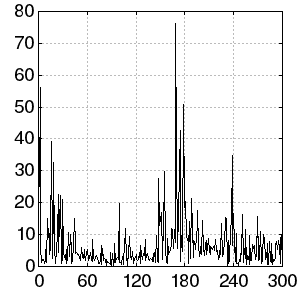
\includegraphics[scale=0.65]{../scripts/brainwaves/wave1.png}
    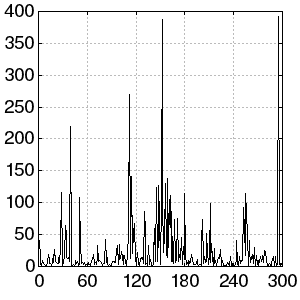
\includegraphics[scale=0.65]{../scripts/brainwaves/wave2.png}
    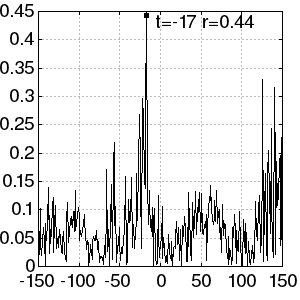
\includegraphics[scale=0.65]{../scripts/brainwaves/result.png}
    \caption{Grafikas kairėje: pirmo dalyvio žemos gama bangos. Grafikas centre: antro dalyvio gama bangos. Grafikas dešinėje: signalų tarpusavio koreliacija. Smegenų bangų signalo stiprumas \(y\) ašyje yra bedimencinis, pagal duomenis pateikusį šaltinį. Ašyje \(x\) - laikas sekundėmis}
    \label{fig:brainwaves}
\end{figure}

Signalų tarpusavio koreliacija turėtų būti stipriausia, kai \( t = 0 \), nes visi dalyviai vienu metu atlieka užduotis.
Bet iš grafiko (~\ref{fig:brainwaves} pav.) matome, kad dižiausias statistinis panašumas yra \( R_{fg}(t) = 0.44 \), kai \( t = -17 \).
Tokie rezultatai gali būti dėl tyrimo metu naudotos netikslios mėgėjiškos įrangos.


    %Conclusions section
    \sectionWithoutNumber{\keyWordConclusions}{conclusion}
    Išvados bei rekomendacijos.


    %file literatureSources.bib
    \referenceSources{literatureSources}

    %% this part is optional
    \newpage
    \begin{appendices}
        \section{Programos kodas}
        \label{app:code}
        \lstinputlisting[language=Haskell]{../../cross-correlation.hs}
    \end{appendices}

\end{document}
